\documentclass[11pt]{article}
%Gummi|065|=)
\title{\textbf{Tecnologico De Jilotepec
\\ }
}
\author{Ulises Isaias Mateos\\
		\\
		\\
		David GR \\
		 \\
		 \\
		Ambar fulrra\\
		\\
		\\
		BetocR7\\
		\\
		\\
		Grupo:3501\\
		\\
		\\}
\date{10/11/2023}

\usepackage {graphicx}
\begin{document}

\maketitle

\section{Introducion de formulas:}


$$1+\frac{1}{1+\frac{1}{5}}$$ \\

$$\frac{-b\pm\sqrt{b^2-4ac}}{2a}$$ \\

$$sqrt 5=1+\frac{1}{1+\frac{1}{1+\frac{1}{1+\frac{1}{\ddots}}}}$$

Matrices\\

$$\pmatrix{3&52&300\cr 41&2&x^2\cr 50&70&90}$$ \\

$$\pmatrix{3&52&300\cr 41&2&x^2\cr 50&70&90\cr 300&100&200}$$ \\


$$
\bordermatrix{
&&& j && K\cr
& 1\cr
&& \ddots\cr
I &&& 0 && 1\cr
&&&&\ddots\cr
K &&& 1 & 0\cr
&&&&&&\ddots\cr
&&&&&&&1}
$$


{
Latex nos permite trabajar con formulas de una manera eficiente, a continuacion vamos a incluir imagenes: dentro del cuerpo del documento, a pie de pagina y encabezado de pagina
}

\begin{figure}
\centering {figure}
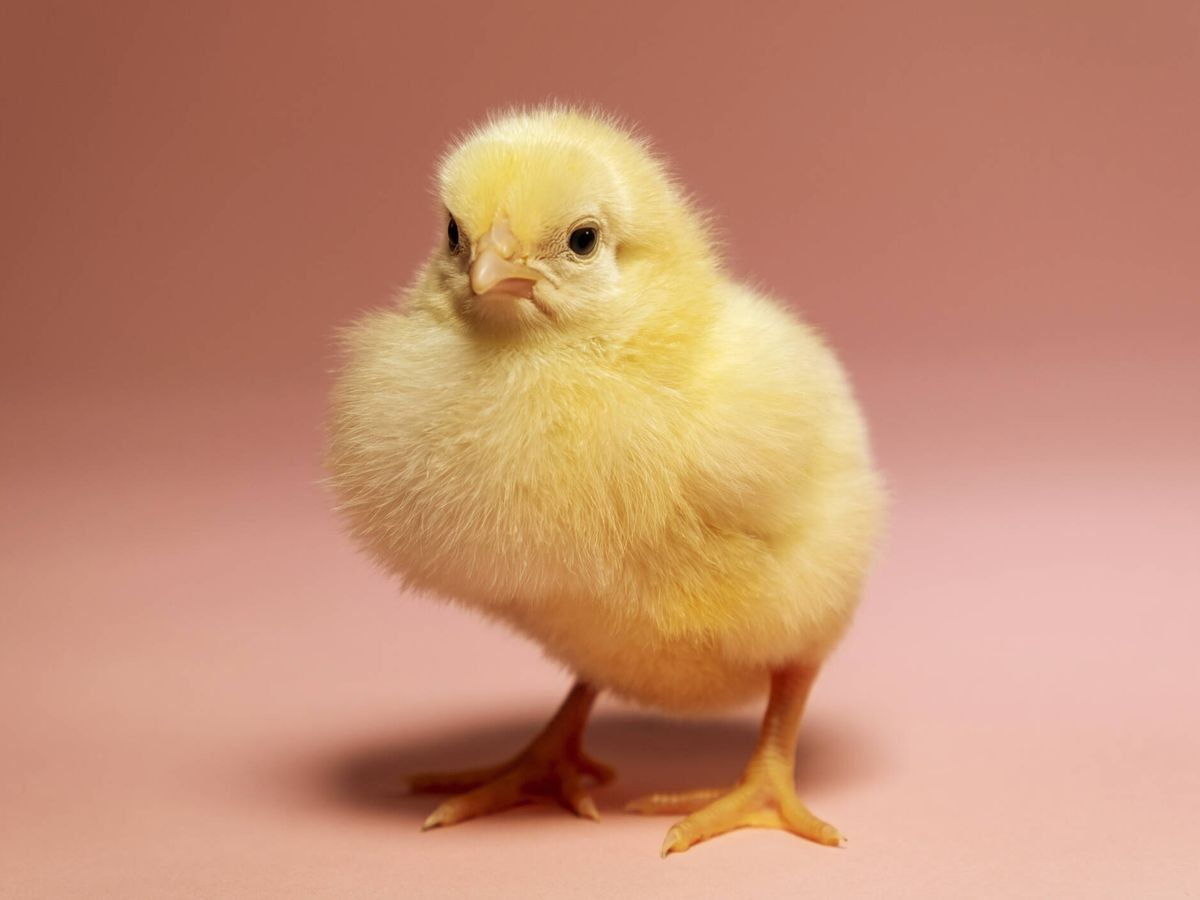
\includegraphics {ww.jpg}\\
\caption {Mi figura}
\label {fig. ejemplo}
\end {figure}






Support for two high-level {\LaTeX} building systems, \emph{rubber}\footnote{https://launchpad.net/rubber/} \& \emph{latexmk}\footnote{http://www.phys.psu.edu/{\textasciitilde}collins/software/latexmk-jcc/} has been added as well. Your preferred typesetter can be configured through the Compilation tab in the Preferences menu. Typesetters that are not installed on your system will not be selectable. 

Added for your viewing convenience is a continuous preview mode for the PDF. This mode is enabled by default, but can also be disabled through the \emph{(View $\rightarrow$ Page layout in preview)} menu. Complementary to this feature is SyncTeX integration, which allows you to synchronize the position in your editor with the PDF preview. 

\section{Feedback}
We hope you will enjoy using this release as much as we enjoyed creating it. If you have comments, suggestions or wish to report an issue you are experiencing - contact us at: \emph{https://github.com/alexandervdm/gummi}.

\section{One more thing}
If you are wondering where your old default text is; it has been stored as a template. The template menu can be used to access and restore it. 

\end{document}

